\section{Kommunikation}

\subsection{Transaktionen}
\todo[inline]{Transaktionen}

\subsection{Sicherheit}
\todo[inline]{Sicherheits}

\subsection{Authentifizierung mit OAuth}
\label{oauth}

\todo[inline]{OAuth (Login-Flow I und II)}

Die Idee hinter OAuth ist bestechend einfach: eine Applikation möchte auf Resourcen eines Benutzers bei einem anderen Dienst zugreifen.
Der Benutzer will der Applikation aber nicht sein Passwort verraten, sondern lediglich einige wenige Resourcen freigeben.
Da sowohl der Benutzer als auch die Applikation dem Anbieter der Resource vertrauen, kann der Benutzer seinen Anbieter anweisen der Applikation Zugriff zu gewähren.
Der Anbieter erstellt dazu ein sogenanntes Access Token, welches er der Applikation zur Verfügung stellt.

Dieses Prinzip hat auf den ersten Blick nichts mit einem Login zu tun, jedoch kann das Vertrauensverhältnis des Benutzers zum Anbieter und der Applikation zum Anbieter genau dazu genutzt werden einen Benutzer einzuloggen ohne von ihm ein Passwort zu verlangen. 
Die Resource ist in diesem Fall lediglich die Bestätigung der erfolgreichen Authentifizierung allenfalls weitere Angaben zum Benutzer wie Namen oder ein Profilfoto.

\begin{figure}[H]
	\centering
	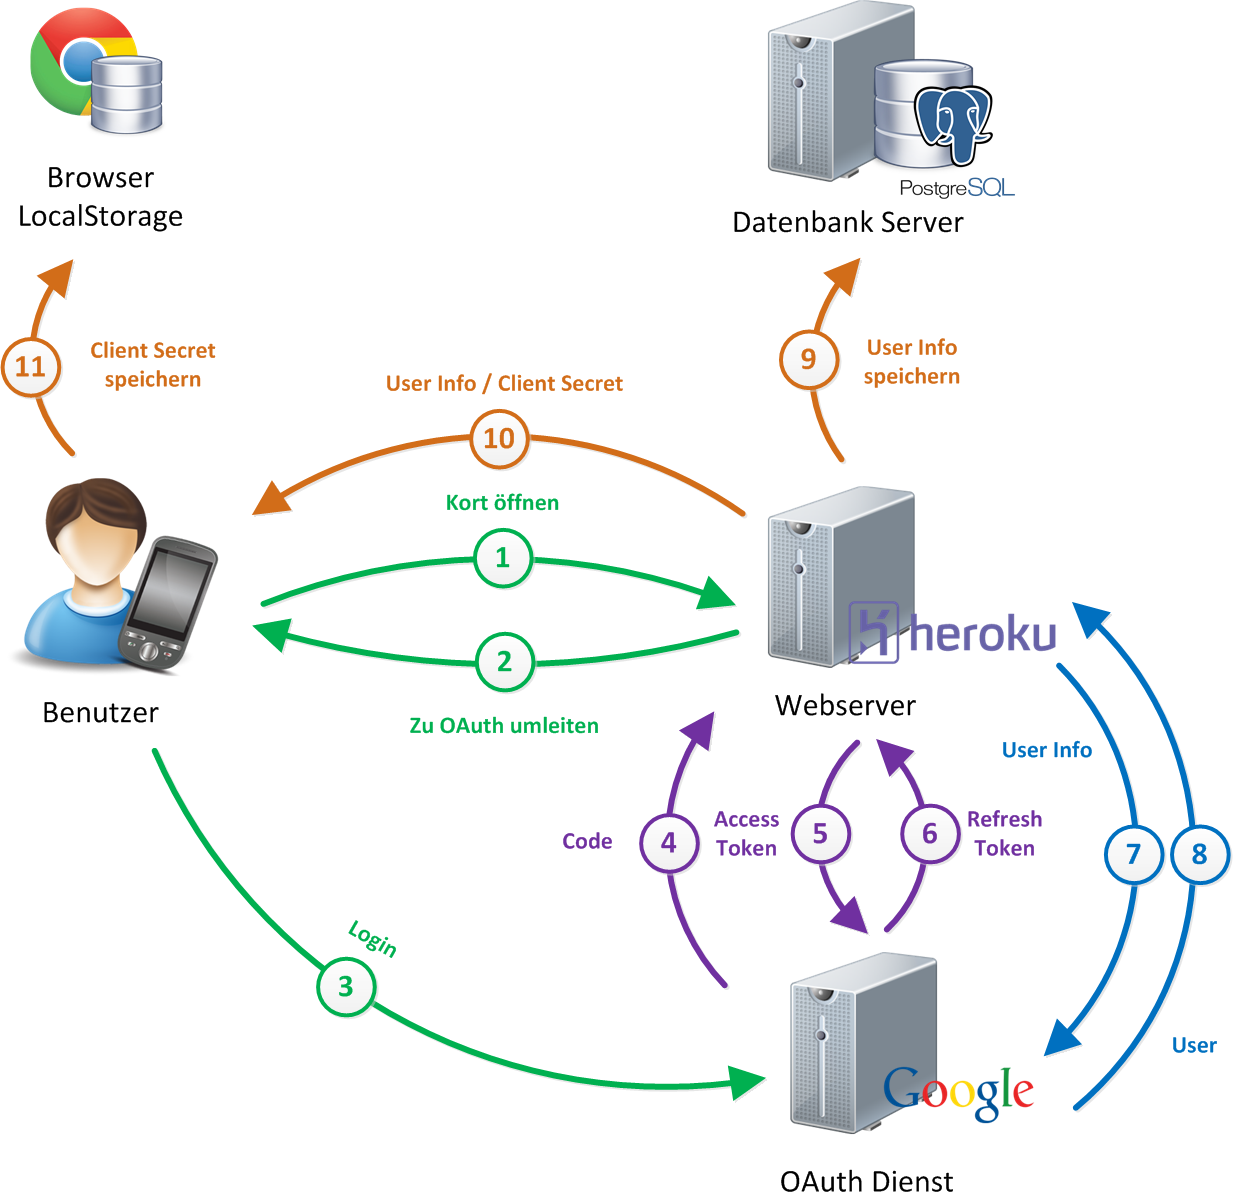
\includegraphics[width=\textwidth]{images/implementation/backend/kort-login}
	\caption{Erster Login des Benutzers mit OAuth}
	\label{image-kort-login}
\end{figure}

In unserem Fall ist \textsc{Kort} die Applikation und Google der Anbieter der \emph{Benutzer}-Resource.
Um dem Benutzer zu ersparen sich bei jedem Besuch erneut via OAuth anzumelden, wird auf dem Server ein \emph{Secret} generiert.
Dieses wird lokal beim Benutzer gespeichert und ermöglicht es dem Benutzer beim nächsten Login direkt dieses Geheimnis zu übermitteln um Zugriff zu bekommen.
Diese Übertragung sollte wenn möglich über SSL/TSL erfolgen.

Wenn der Benutzer erfolgreich eingeloggt wurde, wird dies direkt in der Session des Benutzers gespeichert.
Auf die entsprechenden Werte wird dann bei sicherheits-kritischen Abfragen zurückgegriffen.
So ist sichergestellt, dass ein Benutzer auch wirklich nur seine eigenen Daten manipulieren kann.

\begin{figure}[H]
	\centering
	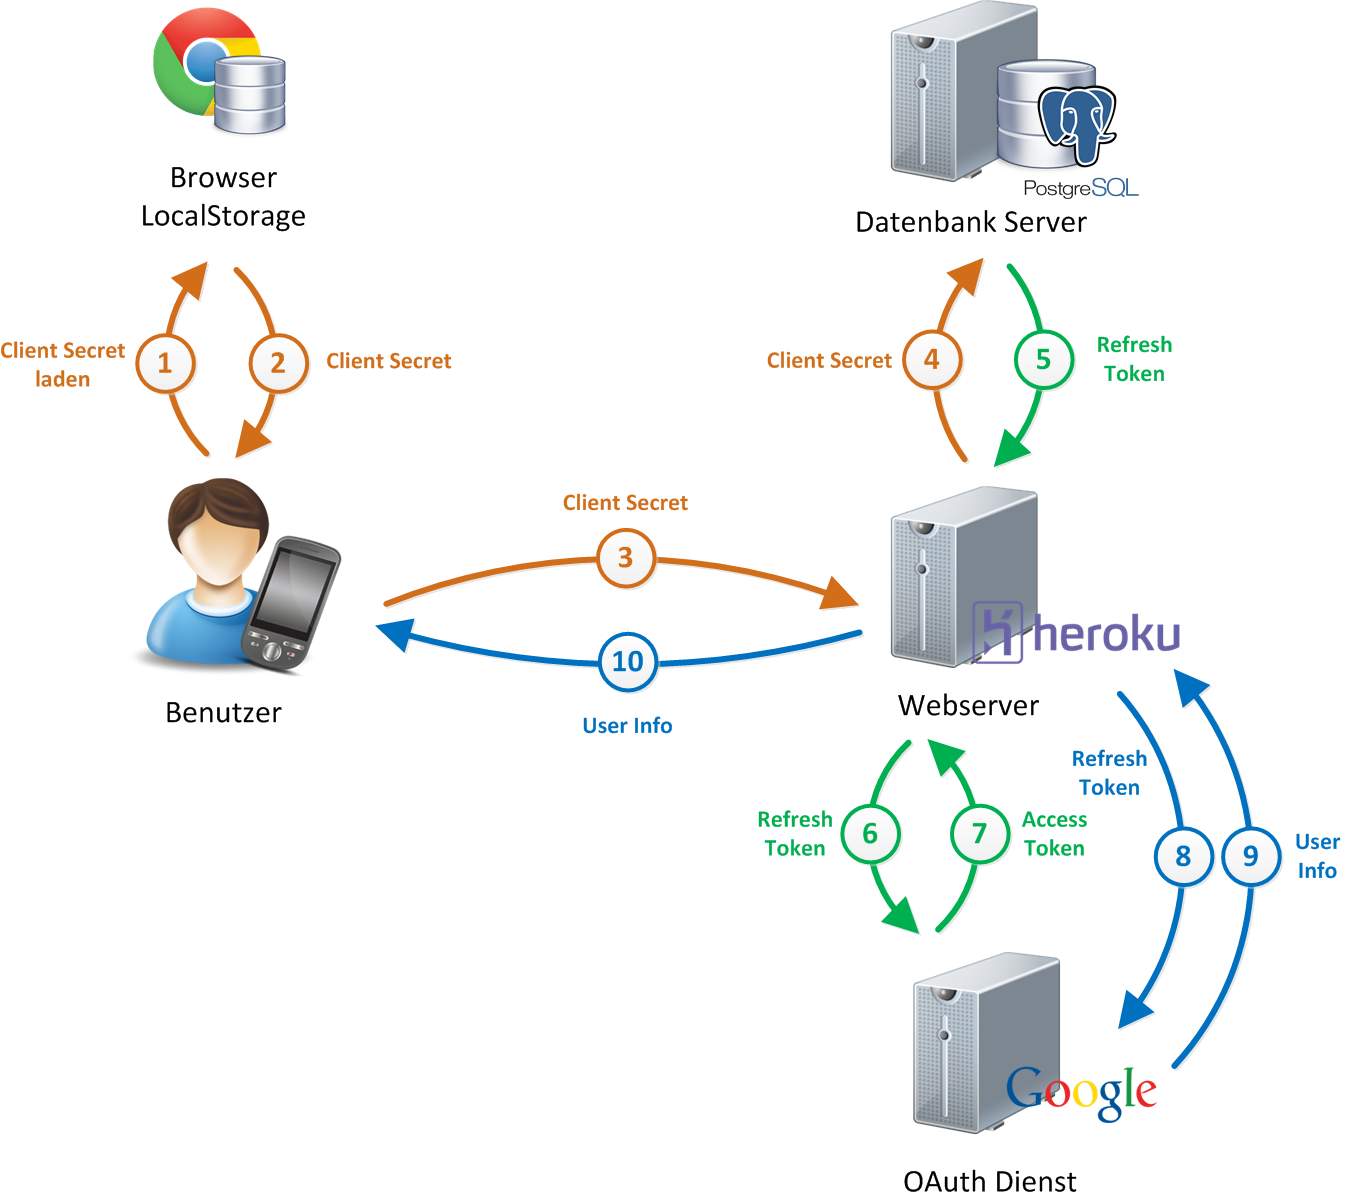
\includegraphics[width=\textwidth]{images/implementation/backend/kort-relogin}
	\caption{Wiedererkennen des Benutzers ab dem zweiten Login}
	\label{image-kort-relogin}
\end{figure}

\subsection{Registrierung der Applikation bei Google}
Um den Google OAuth Dienst zu nutzen, muss diese zuerst registriert werden.
Um einen Benutzer einzuloggen wird er von \textsc{Kort} zu Google weitergeleitet.
Von dort wird er dann nach erfolgter Authentifizierung wieder zurückgeleitet.

Dieses "Zurückleiten" wird auch als \emph{Callback} bezeichnet.
Bei der Tegistrierung müssen die gültigen Werte für den Callback definiert werden.

\begin{figure}[H]
	\centering
	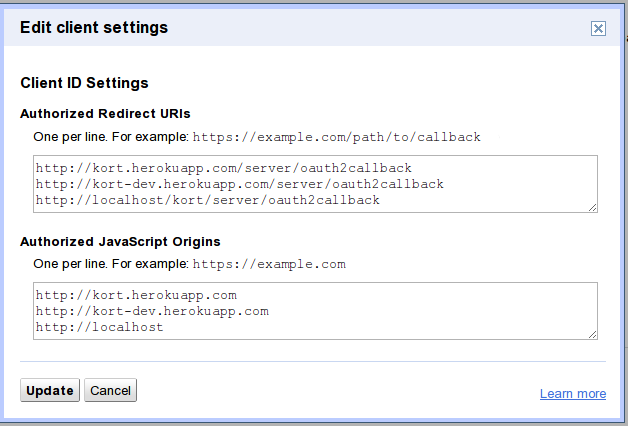
\includegraphics[scale=0.5]{images/implementation/backend/oauth-google-settings}
	\caption{OAuth Einstellungen}
\end{figure}